\subsection{IV Saver} \label{subsec:IVSA}
In this section the IV Saver will be described. The IV Saver, or IVSA for short, is tasked with allocating an address to incomming samples, hence the name IV Saver, it "saves" current I and voltage V at a specific address. The whole system is configured to save current at even addresses i.e. 0, 2, 4, 6 etc. and voltage at uneven addresses i.e. 1, 3, 5, 7 etc. "one sample" consists of two 16 bit values, one for current and one for voltage, so for each sample, the IVSA module recieves two 16 bit words that must be stored. An address is simply assigned to each incomming 16 bit word by a counter. Thus when the first value enters, that is a current, it will be given address 0, and the counter increases by one, the next value to be stored is a voltage, and this will automatically be given address 1. The next value will then be from the next sample, and the first value will be a current, and this is then allocated address 2, the next value is a voltage that is then given address 3, and so on. The interfaces between the IVSA and other modules can be seen in appendix \ref{App:IVSA_INTERFACE}.

In addition to allocating address to incomming current and voltage samples, the IVSA module also acts as a MUX. When the system is in busy mode, i.e. sampling, it will connect the incomming sample values to the Memory Distribution Module and disconnect the IXMUX from this module. This results in the MCU not being able to fect sample data when the system is sampling. Once the system enters done mode, and has reached the desired number of samples, the IVSA connects the IVSA to the Memory Distribution Module, allowing the MCU to fetch the sample data having been stored in the external memory. 

The IVSA moule also control wheter data is to be read from external memory or written to it. When the system is in busy mode, the IVSA will tell the Memory Distribution Module to enter write mode, as sample data most be stored. When the system is in done mode, the IVSA will tell the Memory Distribution Module to enter read mode, as the MCU is expected to fetch the sampled data stored in the external memory.

\subsubsection{Read/Write addressing}
To control the addressing of the incomming data, and the fecthed data the IVSA uses two functionally identical counters. The VHDL code for the counter that allocates an address to the incomming sampled data can be seen in listing \ref{lst:7_2_4_IVSA_SMPL_COUNTER}. Here it can be seen that if reset is a logical 1 or the system enters done mode, the sample address counter is set to 0.

When the system is in busy mode, it will on each falling edge of the input "i\_ADC\_DATA\_RDY" increase the sample counter by one. The data to any given address is clocked in on the rising edge of "i\_ADC\_DATA\_RDY" by the Memory Distribution Module, thus by increasing the address on the falling edge, data integrity is ensured, such that the address is not changes on the same edge data is clocked in.

\lstinputlisting[language=VHDL ,style = c,firstnumber=1, linerange=106-117, caption={Address counter for the sampled data.}, label={lst:7_2_4_IVSA_SMPL_COUNTER}]{Sections/7_SystemDesign/Code/IV_SAVER.vhd}

listing \ref{lst:7_2_4_IVSA_FETCH_COUNTER} shows the counter used for addressing when data is to be fetched from the external memory. The only difference here being that the counter only resets if reset is set to a logical 1. When the system is in done mode, the IVSA indicates to the Memory Distribution Module that it shall be configured for read opperation. When the MCU then sends a clock the IVSA will feed this clock through to the Memory Distribution Module, and the Memory Distribution Module will then fetch whatever data is present on the given address, this data will then be directed through the IXMUX to the IO port and finaly to the MCU. Here the address increases on the falling edge to ensure that the address does not change will the data is being fetched. 

\lstinputlisting[language=c ,style = c,firstnumber=1, linerange=119-130, caption={Address counter for the fetch data cycle.}, label={lst:7_2_4_IVSA_FETCH_COUNTER}]{Sections/7_SystemDesign/Code/IV_SAVER.vhd}

\subsubsection{IVSA MUX opperation}
When the system is in sample mode, the IVSA will as mentioned route the "i\_ADC\_DATA\_RDY" and "i\_DATA" signals through the IVSA to the Memory Distribution Module, as well as assign an address to the incomming data. The MUX for this can be seen in listing \ref{lst:7_2_4_IVSA_SMPL_MUX}. 

\lstinputlisting[language=c ,style = c,firstnumber=1, linerange=90-104, caption={Sample mode MUX}, label={lst:7_2_4_IVSA_SMPL_MUX}]{Sections/7_SystemDesign/Code/IV_SAVER.vhd}

The MUX for read mode can be seen in listing \ref{lst:7_2_4_IVSA_READ_MUX}.
\lstinputlisting[language=c ,style = c,firstnumber=1, linerange=133-148, caption={Sample mode MUX}, label={lst:7_2_4_IVSA_READ_MUX}]{Sections/7_SystemDesign/Code/IV_SAVER.vhd}

These two muxes can be decribed by a simple dataflow diagram as seen in figure \ref{fig_7_2_4_IVSA:MUX}.

\begin{figure}[H]
    \centering
    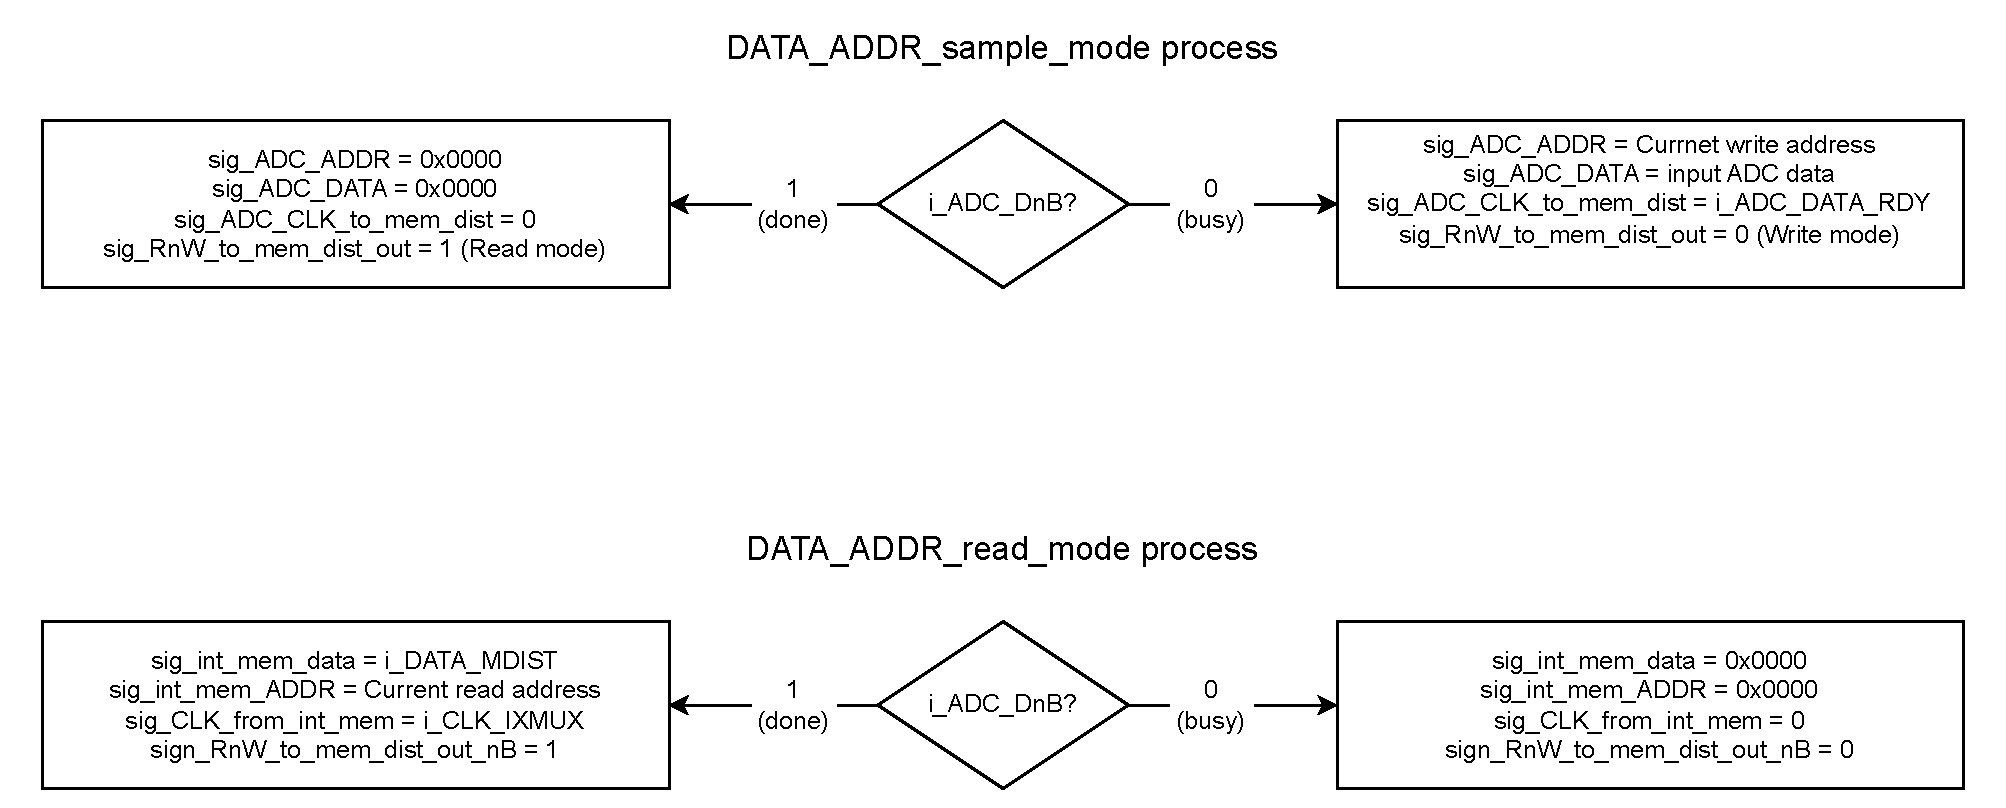
\includegraphics[clip, trim=0 0 0 0, width=1\textwidth]{Sections/7_SystemDesign/Figures/SMPLT_MUX.pdf}
    \caption{A dataflow diagram of the IVSA MUX opperation.}
    \label{fig_7_2_4_IVSA_MUX}
\end{figure}

The output of these two MUXes is then combined to a single output to the memory distribution by a simple "or" function, this can be seen in listing \ref{lst:7_2_4_IVSA_OUT}. Notice that no logic function is performed on sig\_INT\_mem\_DATA is and sig\_ADC\_DATA, as the IXMUX will never write data to the external memory, there is no need to route the output data to the Memory Distribution Module to the IXMUX, and the ADC data is never to be directly routed to the IXMUX, so the only data that is no flow from the IVSA to the IXMUX is that from the external memory.

\lstinputlisting[language=c ,style = c,firstnumber=1, linerange=74-79, caption={Combining the muxes sample mode MUX and read mode MUX to a single output to the Memory Distribution Module.}, label={lst:7_2_4_IVSA_OUT}]{Sections/7_SystemDesign/Code/IV_SAVER.vhd}

At this point it should be noted that more elegant solutions exist, this however works, and given the time limit, it was deemed unecesary to simplify and polish this module. A single MUX together with the address counters could do the same job.